% $Id: finalreport.tex 4414 2013-02-11 10:48:35Z jabriffa $

\documentclass{surreydissertation}
\usepackage{booktabs}
\usepackage{array}
\usepackage{float}
\usepackage[table,xcdraw]{xcolor}
\usepackage{tabu}
\usepackage{microtype}
%\usepackage[T1]{fontenc}
\usepackage{geometry}
\usepackage{listings}
\geometry{a4paper, margin=1in}
\usepackage[table]{xcolor}
% Added this as I would get bitmapped Computer Modern on Windows
\usepackage{lmodern, changepage} % this does mean the names list becomes two lines long, so I fixed it with changepage package
\usepackage{colortbl}
\usepackage[nameinlink]{cleveref}
\definecolor{dustygreen}{HTML}{8A8776}

\title{NLP Group Coursework}
\author{Anna Carter, Evan Williams, Melric Lazaro, Zion Ejechi}
\urn{6702876, 6673385, 6695534, 6687869}
\date{May 2024}
\degree{Natural Language Processing (COM3029)}
\supervisor{Dr. Diptesh Kanojia}

\begin{document}
\maketitle

\tableofcontents
\newpage

\section{Introduction}
As part of the group coursework we came together as a group to deploy Conditional Random Field (CRF) as our model for the Web Application. We explored several service options to facilitate the deployment and discussed the integration and setup of multiple components including the backend configuration, front-end application and API considerations. Furthermore we evaluated the scalability and efficiency of our deployment under stress conditions to ensure its availability and reliability. Since our current model is relatively small in terms of demand for resources we consider smaller options. However we also explored services with more powerful resources to enable future scalability as our model grows. 

\section{Review of Serving Options}
To host our NLP model so that users can interact with it, we considered several serving options that could suit our needs taking into account cost, ease of use, flexibility and future scalability discussed below. In an ideal scenario, users should be able to contact the backend model, hosted on a server in the cloud, containing the input sentence that they want BIO tags to be generated from however we must also account for cost, set-up and maintenance complexity. This discussion will help us deploy our model with the most appropriate serving option.


\subsection{Cloud-based Services}
Firstly, we considered the cloud-based service AWS SageMaker~\cite{AWSSageMaker} which provides services for training, deploying and testing of machine learning models. This service is robust and enables it to run at scale due to the resources available. Furthermore it seamlessly integrates with other AWS features offered to further scale and add additional functionality. However, these resources come at a cost and incur high server fees which can get expensive depending on the methodology used. Furthermore, the complexity managing the cloud architecture requires expertise.

\subsection{Specialised Model Serving Frameworks}
We also considered specialised model serving frameworks like TorchSave~\cite{TorchSave}, TensorFlow Serving~\cite{tensorflow}, Hugging Face~\cite{huggingface} and StreamLit~\cite{streamlit}. These are usually more tailored for specific tasks or domains. Furthermore we discussed various API frameworks to complement our understanding before making a final decision. 
%TODO Perhaps reword this?
They are a bit more niche and specialised, like Tensorflow is a specialised one used to help Tensorflow models or like they have specialised features whereas others are more generic and can be more flexible but less niche if that makes sense. 

\subsubsection{TorchSave/TensorFlow Serving}
TorchSave and TensorFlow Serving both provide flexibility for these models to run efficiently specifically in a production environment. These services are dedicated to specialised model serving so the set up requires specific knowledge and expertise adding to the complexity where other models may be simpler and offer a similar performance.

\subsubsection{Hugging Face}
Another consideration was Hugging Face for hosting the service as it also provides a simpler solution for development and deployment. The main issue with this approach is that it places a middleman between the service and the user, with the latter needing to go through Hugging Face to make requests to the model. This would imply that Hugging Face could act as a weak link and if their servers are unavailable, users will not be able to interact with the model to no fault of our own. Additionally, Hugging Face places their own restrictions on API usage which can further limit availability.

\subsubsection{StreamLit}
StreamLit offers an all-in-one solution for development and deployment of the service, along with acting as its own CI/CD solution by having its own repository style system for maintenance, saving time and efforts which can be used elsewhere. Additionally, StreamLit also allows for easy creation of a user-friendly front-end which can interact directly with the model. Due to the structure of the API, built in components are tightly coupled therefore making it less flexible and harder to debug if there is an issue with a single component. If we build this out in the future this solution would not be appropriate.

\subsection{Container-based Deployment}
Container-based solutions such as Docker or Kubernetes are also flexible and scalable. Kubernetes is more scalable than Docker and offers automated deployment whereas Docker is simpler to set up. Using Docker for initial deployment would eliminate server fees and simplify the set up because this would not require any additional knowledge of cloud technologies such as AWS and Azure~\cite{azure}.

\subsection{API Considerations}
Flask~\cite{flask} acts as a lightweight solution and easy solution which is good for working with proof of concepts. It has minimal overhead and simple to implement so developers can develop applications quickly. An alternative to this would be using frameworks such as Django, however, this is more commonly used for fully fledged web applications and requires more time and setup to get working for deployment but can be a good path if we decide to scale the project up to be more functional through multiple pages and other functions. FastAPI~\cite{fastapi} was also considered as an alternative however integrating it requires more developmental work and there are others such as Flask that are more suitable for our task to save time.

\subsection{Our Choice}
We evaluated several service options for hosting our NLP model. At the moment, since our model is small, we can't justify the expense and complexity of configuring it on AWS. So we decided to avoid using cloud-based services for now. Furthermore, we found that the specialised frameworks we considered weren't tailored for web applications and instead they were more focused towards model deployment. Therefore, we decided not to use them. We chose to use Flask for the backend due to its simplicity to configure and cost effectiveness. This application is suitable for models that are proof-of-concept models or prototypes and require fewer resources. We decide to use Docker as it is simple to set up and offers the environment for users is consistent. However the main issue with using Docker is that each user will be using a different hardware setup, meaning that inference times can vary significantly. Despite this, we used Docker for its simplicity and suitability for our model as a prototype and felt this was the best choice. In the future, as our model base grows, we can consider scaling the work up using cloud services to enable more workload. 

\section{Deployment of the Service}
\label{sec:deployment}
In this section, we discuss the web service implementation, the components that make up the system and the architecture we used in deployment. More specifically we discuss the set up and workings of the front-end system, its interface and how to use it. We discuss the technical components of the backend that serve as a middleman between the interface and the model to get predictions for the user. We also describe the CRF network we built and deployed to inference and obtain predictions. Finally, we discuss Docker and how we used it to set up the environment for containerising the application.

\subsection{Overview of the System}
\label{sec:system-overview}
We have chosen the Flask application service and Docker container to host our model locally. The components  shown in Figure~\ref{fig:NLPsystemoverview2} of the deployed system include a simple front-end application, that sends a sentence in a request to the backend application to receive the predicted NER tags. The backend system composed of Flask and Python requests the predictions from the model which then returns this back to the application which in turn uses the Flask API to send the prediction as a response back to the user.


\begin{figure}
    \centering
    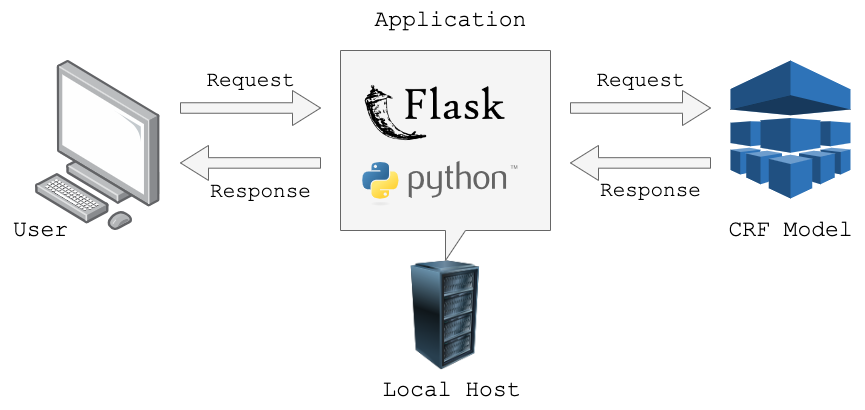
\includegraphics[width=0.9\linewidth]{Figures/NLPsystemoverview2.png}
    \caption{Overview of System}
    \label{fig:NLPsystemoverview2}
 \end{figure}

\subsection{System Pipeline}
The system pipeline shown in Figure~\ref{fig:NLPsystemoverview1} consists of a user sending a request to the server in the form of the sentence to tag with B-O labels. This is then pre-processed by the application using tokenisation and other methods which is then sent to the model for inferencing. Once the model has generated the output, it is converted to JSON which is then sent via POST back to the user in the front-end and is finally displayed to the user.

\begin{figure}
    \centering
    
\includegraphics[width=1\textwidth]{Figures/NLPsystemoverview1.png}
    \caption{Request to Server Process}
    \label{fig:NLPsystemoverview1}
 \end{figure}

\subsection{Environment Set Up}
The environment requires an installation of Docker to run and set up the service on a local machine. Additionally, Python 3.11, the latest version of Flask and the spaCy tokeniser is required to run. These installations are handled when the command \texttt{Docker compose up –-build} is run with the full instructions to prepare the environment found in the Docker file in the codebase repository. Once the Docker container is running, the service can be found on port 8000 of localhost. 

%\subsection{Backend Methodology}
\subsection{Initialisation and handling user input}
When the service starts, Flask initialises the CRF model using the saved weights from training, stored in the Pickle format. At the same time, the templates used to display the frontend are loaded. When a user types a sentence on the home page and presses submit, this string is converted to JSON and is sent back to the server using its dedicated URL using POST as part of the API. Once the server retrieves the request at the URL, the sentence string is decoded from JSON back to plaintext along with recording the current time and date which is used for logging such events. The string is then passed to the prediction function which manages pre-processing that is required for inference with the CRF.

\subsection{Preprocessing}
For a more intuitive experience, users can input a sentence in plaintext used to retrieve the required BIO tags. As the CRF model underneath cannot interpret this directly, the system needs to pre-process this data so that it can be used for inference. When the sentence is sent to the preprocessor, it is first split into tokens using the tokeniser found in the spaCy library. As we are working with a CRF, the tokeniser does not need to add special tokens which are required for transformer models.While this set of tokens can be directly sent to the CRF model, to achieve better prediction accuracy, the system also generates a set of features for each word in the sentence such as checking for capitalisation, prefixes, suffixes, and symbols for example.

\subsection{System}
\label{sec:system}
The features of the sentence along with its tokens are then sent to the CRF model. Once predictions have been generated, they are once again converted to the JSON format which is then returned to the front end to be displayed.For monitoring purposes, the original unparsed sentence, tokens, predictions, and the current time is written to a CSV file which can be used for debugging and maintenance purposes along with allowing for detections for faults with the system.

\subsection{Frontend Methodology}
The front-end is handled using templates as part of Flask, promoting the usage of DRY techniques by using base HTML and CSS files which can be repeated throughout the website without needing to change the same code in multiple places in case a change is to be made globally. For a user to get predictions from the model, they interact with a form that allows for basic text input. When it is submitted, an AJAX request is made to the corresponding function at the server using its specific URL. When a successful response is retrieved, the returned JSON data is parsed containing the tokens and predictions. Using this data, AJAX dynamically updates the webpage by populating a table by iterating through the two arrays and adds each element to their rows to distinguish them clearly. AJAX then updates the contents of this table, giving instant feedback to the user in addition to handling multiple requests made by the user.

\subsection{User Interface \& User Experience}
To make the front-end more user friendly, the popular and well documented Bootstrap 5 framework is used which provides easier support for building mobile friendly and responsive websites. As most devices on the internet are mobile devices, focusing on this audience allows for the service to reach more users, rather than just desktop users. Additionally, Bootstrap provides standardised elements such as form controls, alongside visually appealing CSS styles, improving user retention, in addition to making the website more accessible by using colour-blind friendly components.
%TODO is it really colourblind friendly?
All of which further streamlines its development as it is widely compatible across browsers.


\section{Evaluation of the Service}
\label{sec:eval}
In this section we critically evaluate the performance of the service. We perform stress testing with various request sizes to identify how many requests the model can handle. We also assess the speed it comes back using browser developer tools. We then justify if this is an acceptable limit for us. We don’t expect perfection, but we justify the threshold through common sense and referencing. To enrich the evaluation, we also perform error analysis techniques to identify the areas of limitation. For example, how many times a feature or function fails, where it fails and the reasons why it fails. Furthermore, we discuss the scalability of the system, assessing its suitability with larger language models. We consider the below points as part of our evaluation criteria:

\begin{itemize}
    \item To perform stress testing, we send a stream of concurrent requests systematically to the backend and evaluate the success of the response and inference time to get a reply.
    \item We acknowledge that request times may not be fixed due to the differences in hardware when the Docker container is distributed to users and hardware resources available.
    \item When deployed on the server, this hardware will be more consistent so we can expect the same results under the same conditions used for the stress testing.
\end{itemize}

\subsection{Performance Evaluation Methods}
For evaluation, a combination of spike testing and ramp testing using POSTman~\cite{postman} was performed to evaluate the performance of the service. The spike testing is performed by sending a low number of requests to the server and then sending a high number of requests all at once at a given point in time over the period of one minute. This shows how the model performs when a small group of users make several requests to the server together. Ramp testing involves increasing the number of requests in the period of one minute to see how the server deals with a continuous load, mimicking how users will interact with the service if it were to be deployed on a large-scale basis. 

\begin{figure}
    \centering
    \subfigure[Spike Test]{\label{fig:spike}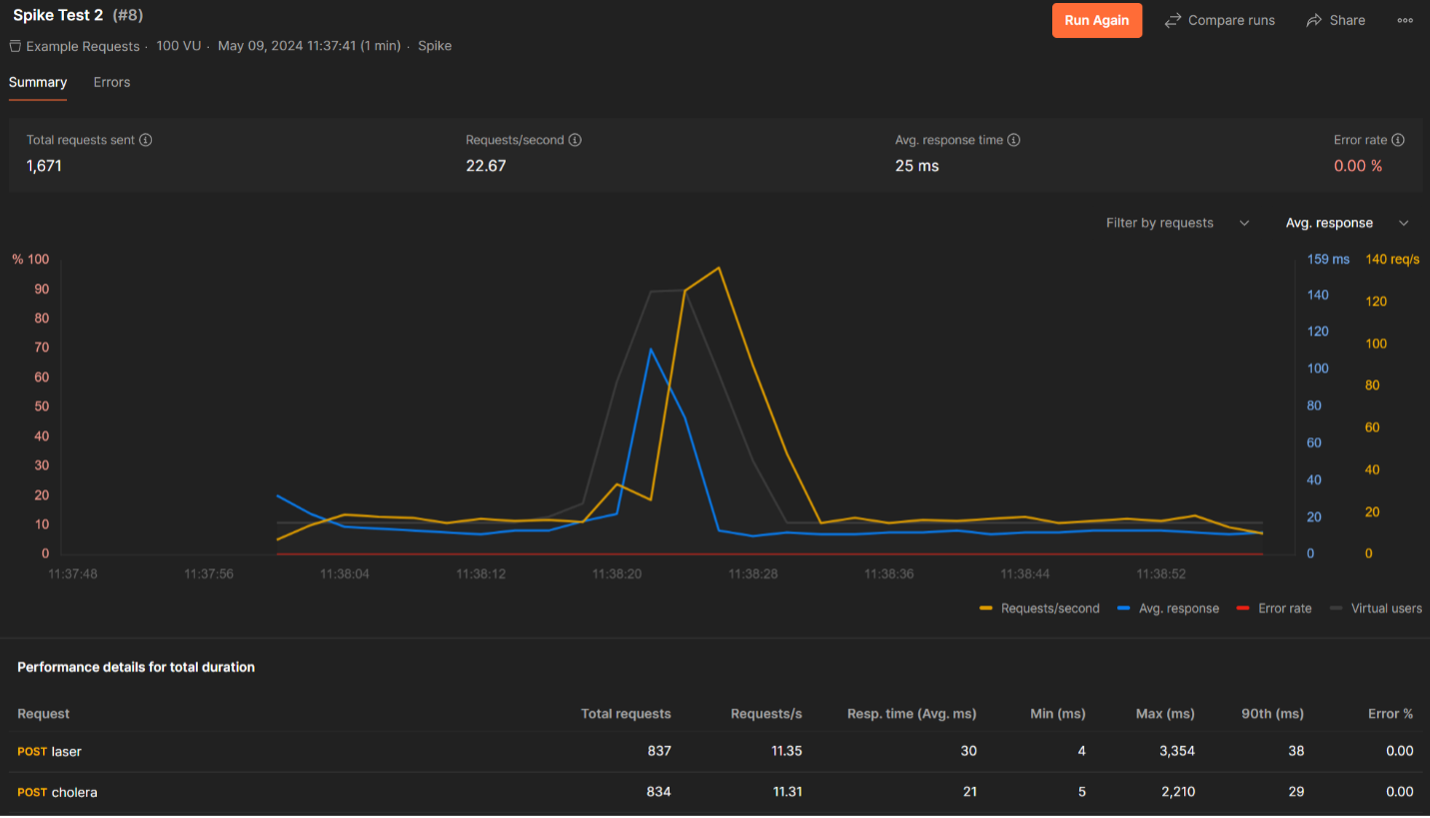
\includegraphics[width=\textwidth]{Figures/spike.png}}
    \subfigure[Ramp Test]{\label{fig:ramp}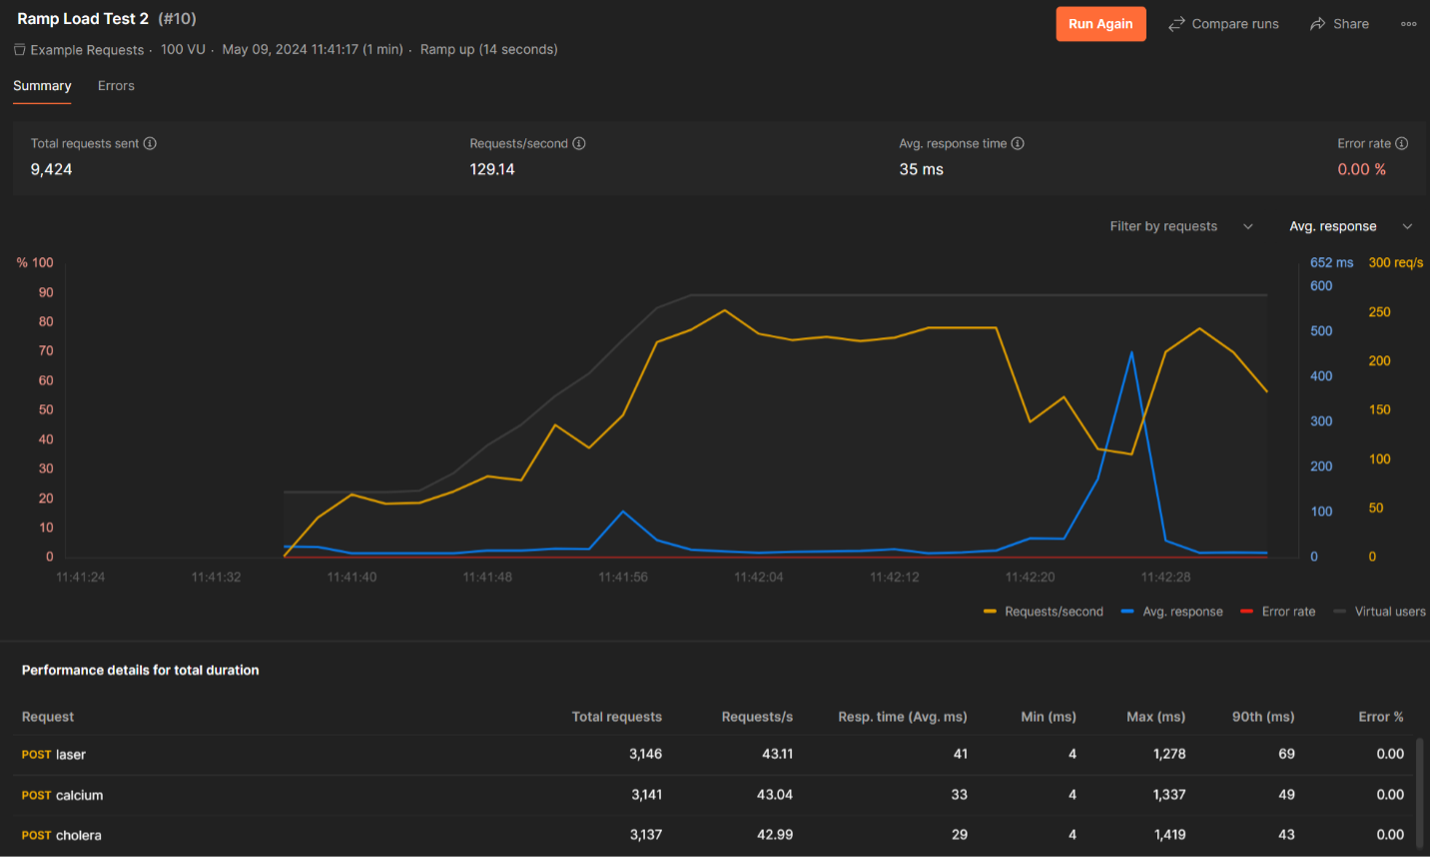
\includegraphics[width=\textwidth]{Figures/ramp.png}}
    \caption{Spike and Ramp results in Postman}
    \label{fig:results}
    \end{figure}

In Figure~\ref{fig:results} the yellow lines represents the number of requests being sent to the server per second with the blue lines representing the average response time. The red lines highlights the error rate seen by the server over this stress test. One limitation with using POSTman for evaluation is that the number of requests is restricted to around 100 virtual users. To see a noticeable difference, we would need to have thousands of virtual users to a noticable difference in terms of error rates. For what is possible, we can see that the architecture is robust for a small number of users. In the future, we could use utilities like celery to handle long running requests and evaluate how the architecture performs and make necessary changes if necessary.

\subsubsection{Spike Testing Analysis}
Looking at the results of the spike test, we can see that under normal conditions, the service responds at an average rate of just under 20ms showing that the combination of running locally along with the architectural choice of using Flask gives real time responses back to the user upon making a request to the server due to it being lightweight and effective enough for the task, minimising computational resources which can be allocated to handling requests. When the spike occurs, the response rate peaks at around 110ms and then quickly recovers back to its usual rate of under 20ms. This may be due to the user’s device allocating more resources for computation, for example, increasing CPU clock rates, which in turn explains the reduction in response time before reaching peak requests. Additionally, for a total of 1671 requests made, the service does not produce any errors showing its reliability.

\subsubsection{Ramp Testing Analysis}
Observing the ramp testing results, we can see that the service struggles more with this. For most of this experiment, the server can handle the increasing load of requests well with only small spikes being observed, jumping to around 100ms like the spike testing results. When peak load is reached and sustained, the server again, mostly handles this well until a point where the average response sees a large spike to around 450ms when load starts to briefly decrease. This could be due to computational limitations being reached along with other background factors in play. Again, we also see an error rate of 0\%, further showcasing its robustness.

\subsection{Endpoint Testing}
As part of our evaluation of the service we conducted various end-to-end tests to assess how the endpoint performs whilst the application is being used. Each test involved sending a request to the server to retrieve information and comparing the actual response with the expected outcome. These tests focused on the boundary conditions of text and validating the input and output. Assertions were made on HTTP status codes and the structure of the responses evaluated to ensure that the API functioned correctly and could handle various input scenarios reliably. The outcomes of these tests, which validated the functionality and reliability of the API, are shown in Table~\ref{tab:testresults}.

\begin{table}
\centering
\begin{tabu} to \textwidth { | X[c] | X[l] | X[c] | X[c] | X[c] | }
\hline
\rowcolor[HTML]{EFEFEF} 
\textbf{Test ID} & \textbf{Test Description} & \textbf{Expected Outcome} & \textbf{Actual Outcome} & \textbf{Status} \\ \hline
1 & Test correct input  & HTTP 200 response & 200 & \cellcolor[HTML]{CCFFCC}\textcolor{dustygreen}{PASS} \\ \hline
\rowcolor[HTML]{E0E0E0} 
2 & Test input above limit (512 tokens) & HTTP 500 response & 500 & \cellcolor[HTML]{CCFFCC}\textcolor{dustygreen}{PASS} \\ \hline
3 & Test empty input string & HTTP 500 response & 500 & \cellcolor[HTML]{CCFFCC}\textcolor{dustygreen}{PASS} \\ \hline
\rowcolor[HTML]{E0E0E0} 
4 & Test shortest input possible & HTTP 200 response & 200 & \cellcolor[HTML]{CCFFCC}\textcolor{dustygreen}{PASS} \\ \hline
5 & Test for all input types & HTTP 200 response & 200 & \cellcolor[HTML]{CCFFCC} \textcolor{dustygreen}{PASS} \\ \hline
\end{tabu}
\caption{Test results for API endpoints}
\label{tab:testresults}
\end{table}

Additionally, during testing we recorded the responses of various input scenarios and provide the examples in Figure~\ref{fig:responses}. When no input is submitted a request is not sent to the server for a prediction as this is an unnessesary computation. Therefore we have implemented error handling and a server error occurs as shown in \Cref{fig:longtext,fig:emptystring} when the input length is over 512 or an empty string is submitted. For optimal user experience the front-end is configured to empty the table as shown in Figure~\ref{fig:reset}.

\begin{figure}
    \centering
    \subfigure[Correct Input Response]{\label{fig:correctinput}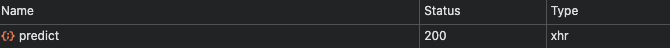
\includegraphics[width=1.0\linewidth]{Figures/correct_input_response.png}}
    \subfigure[Empty String Response]{\label{fig:emptystring}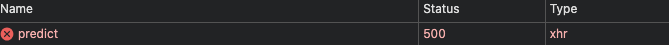
\includegraphics[width=1.0\linewidth]{Figures/empty_string_response.png}}
    \subfigure[Long Text Response]{\label{fig:longtext}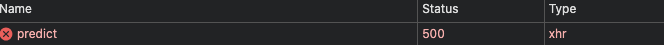
\includegraphics[width=1.0\linewidth]{Figures/long_text_response.png}}
    \caption{Responses from different input scenarios}
    \label{fig:responses}
\end{figure}


\begin{figure}
    \centering
    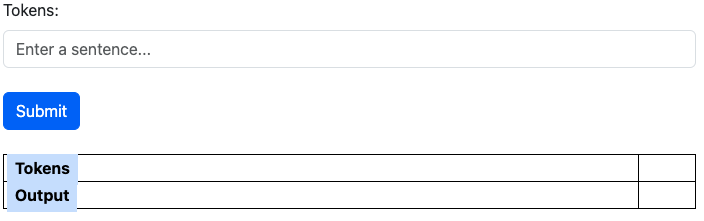
\includegraphics[width=0.6\linewidth]{Figures/emptyfrontend.png}
    \caption{Screenshot of web app showing empty output table}
    \label{fig:reset}
 \end{figure}

\subsection{Impact of Docker Distribution on Performance}
It is important to understand that due to the choice of running locally, hardware may vary across users and different setups may see different results depending on the number of resources available to it, either increasing or decreasing response times respectively. 

As no errors are observed, it may be beneficial to experiment with increasing the number of requests to the server over a longer period to understand the hard limit of the architecture. However, for a small-scale solution, we can see that the current implementation is sufficient.

\subsection{Recommendations for Improving Performance}
To improve the performance, scalability and reliability of the service there are several components that can be improved:

\begin{itemize}
    \item \textbf{Cache:} Implementing a caching system will reduce the workload on the backend because frequently requested results can be stored in the cache reducing the need for resource heavy computations. 
    \item \textbf{Asynchronous Requests:} The efficiency of the service can be improved by implementing asynchronous requests that handle more than one at a time, since there are more responses over time.
    \item \textbf{Load Balancers:} Several load balancers are important to reduce the load on the service and ensure it doesn't get overwhelmed and crash and compromising the applications availability. Nginx is a load balancer that is easy to configure and integrates well with Flask to be used to distribute traffic to and from the application. It is considered suitable for a small system such as the one we have deployed.
\end{itemize}


\section{CI/CD Pipeline and Monitoring}
Continuous Integration and Development (CI/CD) maintains an efficient and reliable working application and considered an important component of the deployment process. We discuss the CI/CD pipeline below along with an explanation of how monitoring is implemented.


\subsection{Build Instructions}
The current implementation of the service is hosted using Docker~\cite{Docker}. The Dockerfile in our repository defines the dependencies, execution commands and environment to run the application. It provides instructions for building a Docker image that contains the application and ensures consistency across different environments. In the file, the base image is specified the as \texttt{python:PYTHON\_VERSION-slim} which contains Python and a slim Linux distribution. Various environment variables \texttt{PYTHONDONTWRITEBYTECODE} and \texttt{PYTHONUNBUFFERED} are set to prevent python writing bytecode files and buffering of standard outputs. Dependencies are downloaded by executing the contents of the \texttt{requirements.txt} file using \texttt{pip install -r requirements.txt}. Port 8000 is defined as the port to listen on and executes the command CMD to run the application using Gunicorn, binding it to the application. Figure~\ref{fig:Docker} shows the status of the Docker container which allows for easy management and observation of performance. 

\begin{figure}
    \centering
    \includegraphics[width=1.0\linewidth]{Figures/Docker.png}
    \caption{Docker Desktop}
    \label{fig:Docker}
 \end{figure}


\subsection{Continuous Integration and Deployment}
Continuous Integration and Deployment (CD) involves automatically testing and integrating code changes into a shared repository. The bash script \texttt{deploy.sh} shown in  Listing~\ref{lst:script}  automates the process of updating the service by downloading and pulling the latest version of the service repository from GitHub and updating the local version, removing any existing Docker containers.  This is done through the command \texttt{Docker compose up --build} that rebuilds the Docker containers defined in the \texttt{Docker-compose.yml} file and starts them up again. This script simplifies the deployment workflow and ensures that the application is always up-to-date and running in a consistent environment.

% Define Bash script style
\lstdefinestyle{bash}{
    language=bash,
    basicstyle=\small\ttfamily,
    keywordstyle=\color{blue},
    commentstyle=\color{gray},
    breaklines=true,
    showstringspaces=false,
    frame=single,
    numbers=left,
    numberstyle=\tiny\color{gray},
    numbersep=5pt,
    backgroundcolor=\color{white},
    tabsize=2,
    captionpos=b,
}

\begin{lstlisting}[style=bash, caption={\texttt{deploy.sh} Bash Script}, label={lst:script}]
#!/bin/bash
set -e

git pull origin main
Docker-compose down
Docker compose up --build
\end{lstlisting}

Furthermore any services that are currently being ran inside Docker are also stopped to maintain integrity of the data being processed. Once safely stopped, a new Docker image is created using the Docker file, building configurations if necessary. This then automatically starts the services required for hosting the model and checks if they are running correctly. This method allows for easy deployment of changes to the service. As this is a manually ran script, this comes with the benefit of additional control and flexibility of deployment. The team can control how the service is deployed to the individual steps and acts as an additional failsafe in case problematic code is accidentally pushed to the main branch. This further protects the users of the service, increasing retention. Its simplicity also allows for immediate feedback as when the script is run, it can be observed whether
%TODO what is "this" referring to?
 this was successful or not and can further identify issues to be resolved. 

\subsection{Monitoring}
For monitoring purposes, as mentioned
%as part of the architecture,
in \autoref{sec:system},
user inputs and model outputs are recorded to a CSV file. This database also records the time of each request and can be used for easy conversion to different data structures which can be used for analysing different parts of the service from the architecture itself to the model. Its simplicity reduces the complexity and time of needing to set up a relational database like SQL and is a lightweight solution, aiding the portability of the service. The data can be viewed by anyone and does not require additional knowledge to understand.

\section{Conclusion and Future Works}
From the findings and observations seen
%previously
in \autoref{sec:eval}, it can be concluded that the currently implemented architecture is fit for purpose for a small-scale proof of concept. The combination of using a generalised framework such as Flask allows for simple development of the service. It also allows for flexibility for scaling up in the future but other frameworks such as Django could be considered if the size of the application were to grow. Figure~\ref{fig:interface} shows the web application interface that is presented to the user.

\begin{figure}[H]
    \centering
    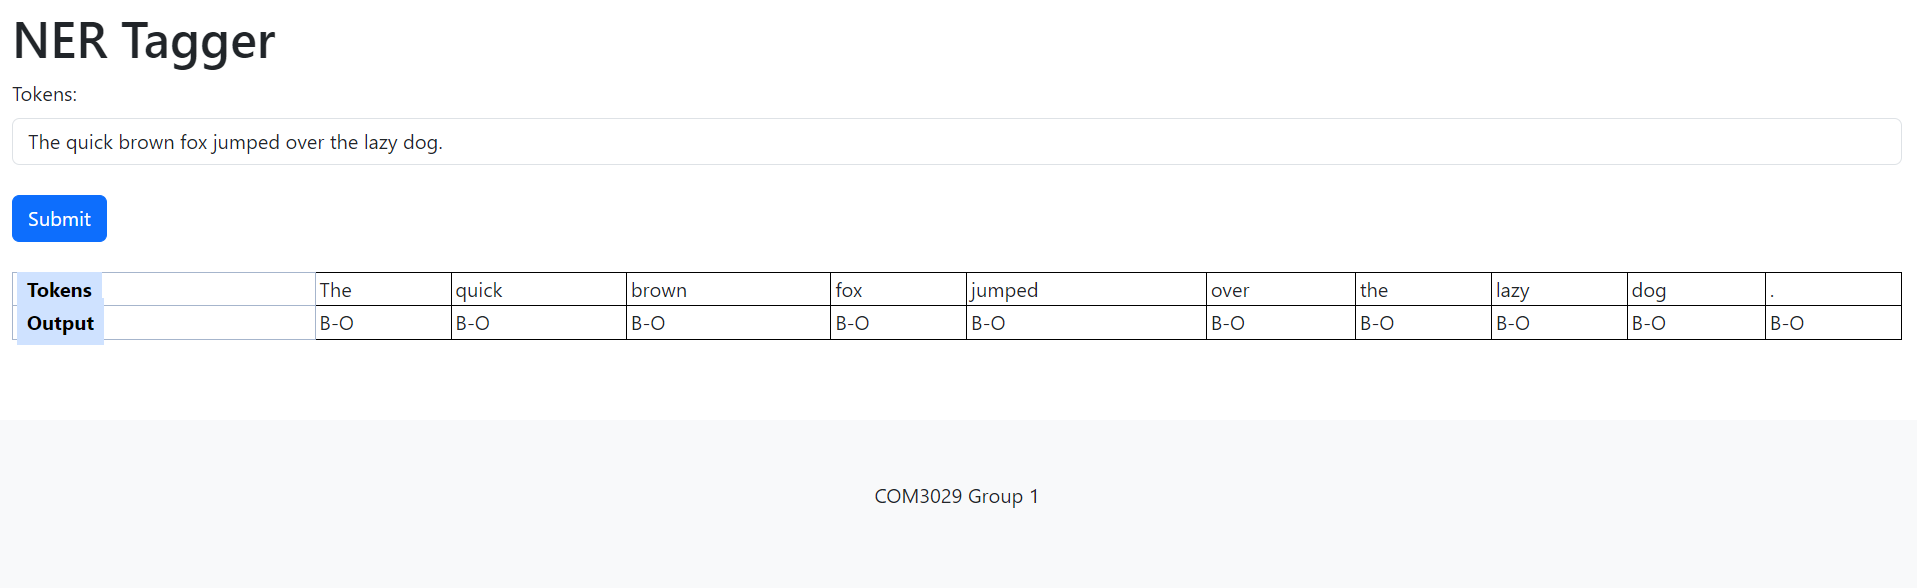
\includegraphics[width=1.0\linewidth]{Figures/frontend.png}
    \caption{Application Interface}
    \label{fig:interface}
 \end{figure}

Through testing, we saw that the architecture is robust enough to handle a moderate number of users making requests in bulk and over a spike. However, to improve these findings, we should attempt to identify the limits of the server by sending the maximum number of requests before errors occur. Using a containerised solution also allows for simple setup of the service on any device and avoids having to pay for additional service fees. Users also can ensure that their data is not stored in a central server and data is instead stored locally to their device, enhancing privacy. If given a budget, cloud solutions may be more viable due to reduced error rates along with handling a larger number of users at once. This can be experimented with in the future.

% appendices
\appendix
%\include{appenda}
%\include{appendb}

\bibliographystyle{agsm}
\bibliography{references}

\end{document}
